\documentclass[12pt,a4paper]{article}

% Packages
\usepackage[utf8]{inputenc}
\usepackage[T1]{fontenc}
\usepackage{lmodern}
\usepackage[margin=1in]{geometry}
\usepackage{graphicx}
\usepackage{xcolor}
\usepackage{listings}
\usepackage{tikz}
\usepackage{pgfplots}
\usepackage{booktabs}
\usepackage{longtable}
\usepackage{hyperref}
\usepackage{fancyhdr}
\usepackage{tcolorbox}
\usepackage{enumitem}
\usepackage{float}
\usepackage{caption}
\usepackage{subcaption}
\usepackage{amsmath}
\usepackage{fontawesome5}

% TikZ libraries
\usetikzlibrary{shapes.geometric, arrows.meta, positioning, calc, decorations.pathreplacing, fit, backgrounds}

% Colors
\definecolor{darkblue}{RGB}{0, 51, 102}
\definecolor{lightblue}{RGB}{230, 240, 250}
\definecolor{darkred}{RGB}{153, 0, 0}
\definecolor{darkgreen}{RGB}{0, 102, 51}
\definecolor{codebg}{RGB}{245, 245, 245}
\definecolor{codeframe}{RGB}{200, 200, 200}
\definecolor{servercolor}{RGB}{52, 152, 219}
\definecolor{clientcolor}{RGB}{231, 76, 60}
\definecolor{datacolor}{RGB}{46, 204, 113}
\definecolor{cryptocolor}{RGB}{155, 89, 182}

% Listings configuration
\lstdefinestyle{cstyle}{
    language=C,
    basicstyle=\ttfamily\small,
    keywordstyle=\color{darkblue}\bfseries,
    stringstyle=\color{darkred},
    commentstyle=\color{darkgreen}\itshape,
    backgroundcolor=\color{codebg},
    frame=single,
    rulecolor=\color{codeframe},
    numbers=left,
    numberstyle=\tiny\color{gray},
    breaklines=true,
    showstringspaces=false,
    tabsize=4,
    captionpos=b
}

\lstdefinestyle{bashstyle}{
    language=bash,
    basicstyle=\ttfamily\small,
    keywordstyle=\color{darkblue},
    backgroundcolor=\color{codebg},
    frame=single,
    rulecolor=\color{codeframe},
    breaklines=true,
    showstringspaces=false
}

% Header/Footer
\pagestyle{fancy}
\fancyhf{}
\fancyhead[L]{\leftmark}
\fancyhead[R]{BlxdMoon Technical Report}
\fancyfoot[C]{\thepage}
\renewcommand{\headrulewidth}{0.4pt}
\renewcommand{\footrulewidth}{0.4pt}

% Hyperref setup
\hypersetup{
    colorlinks=true,
    linkcolor=darkblue,
    urlcolor=darkblue,
    citecolor=darkblue,
    pdftitle={BlxdMoon RAT - Technical Analysis Report},
    pdfauthor={Security Research Documentation}
}

% Custom boxes
\newtcolorbox{warningbox}{
    colback=red!5!white,
    colframe=red!75!black,
    title=\faExclamationTriangle\ Warning,
    fonttitle=\bfseries
}

\newtcolorbox{infobox}{
    colback=blue!5!white,
    colframe=blue!75!black,
    title=\faInfoCircle\ Information,
    fonttitle=\bfseries
}

\newtcolorbox{codebox}[1][]{
    colback=codebg,
    colframe=codeframe,
    title=#1,
    fonttitle=\bfseries\ttfamily
}

\begin{document}

% Title Page
\begin{titlepage}
    \centering
    \vspace*{1cm}

    {\Huge\bfseries\color{darkred} BlxdMoon RAT}\\[0.5cm]
    {\Large\color{darkblue} Technical Analysis Report}\\[2cm]

    \includegraphics[width=0.8\textwidth]{../repo/banner.png}\\[2cm]

    {\large A Comprehensive Study of Remote Access Tool Architecture}\\[1cm]

    \vfill

    \begin{tabular}{ll}
        \textbf{Classification:} & Educational / Security Research \\
        \textbf{Platform:} & Microsoft Windows \\
        \textbf{Language:} & C (WinAPI) \\
        \textbf{Version:} & 2.0 (Multi-Client) \\
    \end{tabular}

    \vspace{1cm}

    {\large\today}

\end{titlepage}

% Table of Contents
\tableofcontents
\newpage

% Warning
\begin{warningbox}
This document is intended for \textbf{educational purposes only}. The techniques described herein should only be used in authorized security research, penetration testing with explicit permission, or controlled laboratory environments. Unauthorized access to computer systems is illegal.
\end{warningbox}

\section{Executive Summary}

BlxdMoon is a Remote Access Tool (RAT) written in C, designed for Windows systems. It implements a client-server architecture where the \textbf{server} acts as a Command and Control (C2) center, and the \textbf{backdoor} (client) executes commands on compromised machines.

\subsection{Key Capabilities}

\begin{itemize}[leftmargin=*]
    \item \textbf{Remote Command Execution} -- Execute arbitrary shell commands
    \item \textbf{File Transfer} -- Upload/download files bidirectionally
    \item \textbf{Surveillance} -- Screenshots, keylogging, clipboard monitoring
    \item \textbf{Credential Harvesting} -- Browser password extraction
    \item \textbf{Persistence} -- Registry-based autorun mechanism
    \item \textbf{Multi-Client Support} -- Manage up to 100 simultaneous connections
    \item \textbf{Encrypted Communications} -- ECDH key exchange + AES-256 encryption
\end{itemize}

\newpage
\section{System Architecture}

\subsection{High-Level Overview}

The following diagram illustrates the overall architecture of BlxdMoon:

\begin{figure}[H]
\centering
\begin{tikzpicture}[
    node distance=2cm,
    server/.style={rectangle, draw=servercolor, fill=servercolor!20, thick, minimum width=4cm, minimum height=1.5cm, rounded corners},
    client/.style={rectangle, draw=clientcolor, fill=clientcolor!20, thick, minimum width=3cm, minimum height=1cm, rounded corners},
    module/.style={rectangle, draw=datacolor, fill=datacolor!20, thick, minimum width=2.5cm, minimum height=0.8cm, rounded corners, font=\small},
    arrow/.style={-Stealth, thick},
    dataarrow/.style={-Stealth, thick, dashed, color=cryptocolor}
]

% Server
\node[server] (server) {\faServer\ \textbf{C2 Server}};
\node[below=0.3cm of server, font=\small\itshape] {Multi-Client Handler};

% Clients
\node[client, below left=3cm and 2cm of server] (client1) {\faLaptop\ Client 1};
\node[client, below=3cm of server] (client2) {\faDesktop\ Client 2};
\node[client, below right=3cm and 2cm of server] (client3) {\faLaptop\ Client 3};

% Network cloud
\node[ellipse, draw=gray, fill=gray!10, minimum width=6cm, minimum height=1.5cm] at ($(server)!0.5!(client2)$) (network) {\faCloud\ TCP/IP Network};

% Arrows
\draw[arrow, color=servercolor] (server) -- (network);
\draw[arrow, color=clientcolor] (network) -- (client1);
\draw[arrow, color=clientcolor] (network) -- (client2);
\draw[arrow, color=clientcolor] (network) -- (client3);

% Encrypted indicator
\node[right=0.5cm of network, font=\small, color=cryptocolor] {\faLock\ AES-256};

% Client modules (for client2)
\node[module, below=0.5cm of client2] (mod1) {Keylogger};
\node[module, left=0.3cm of mod1] (mod2) {Screenshot};
\node[module, right=0.3cm of mod1] (mod3) {Process Mgr};

\end{tikzpicture}
\caption{BlxdMoon System Architecture}
\end{figure}

\subsection{Component Diagram}

\begin{figure}[H]
\centering
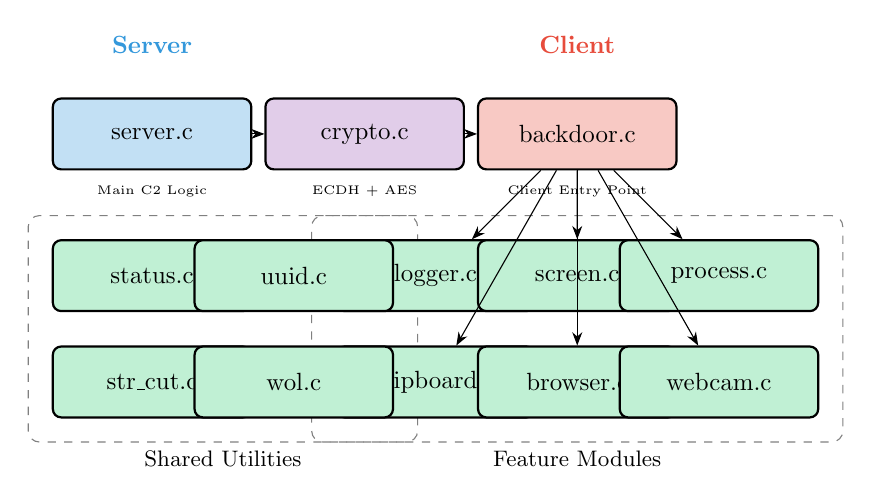
\begin{tikzpicture}[
    scale=0.9,
    transform shape,
    component/.style={rectangle, draw, thick, minimum width=2.8cm, minimum height=1cm, rounded corners=3pt},
    servercomp/.style={component, fill=servercolor!30},
    clientcomp/.style={component, fill=clientcolor!30},
    utilcomp/.style={component, fill=datacolor!30},
    cryptocomp/.style={component, fill=cryptocolor!30}
]

% Server side
\node[servercomp] (servermain) at (0,0) {server.c};
\node[below=0.1cm of servermain, font=\tiny] {Main C2 Logic};

% Client side
\node[clientcomp] (backdoor) at (6,0) {backdoor.c};
\node[below=0.1cm of backdoor, font=\tiny] {Client Entry Point};

% Utility modules
\node[utilcomp] (logger) at (4,-2) {logger.c};
\node[utilcomp] (screen) at (6,-2) {screen.c};
\node[utilcomp] (process) at (8,-2) {process.c};
\node[utilcomp] (clipboard) at (4,-3.5) {clipboard.c};
\node[utilcomp] (browser) at (6,-3.5) {browser.c};
\node[utilcomp] (webcam) at (8,-3.5) {webcam.c};

% Crypto
\node[cryptocomp] (crypto) at (3,0) {crypto.c};
\node[below=0.1cm of crypto, font=\tiny] {ECDH + AES};

% Shared utilities
\node[utilcomp] (status) at (0,-2) {status.c};
\node[utilcomp] (uuid) at (2,-2) {uuid.c};
\node[utilcomp] (strcut) at (0,-3.5) {str\_cut.c};
\node[utilcomp] (wol) at (2,-3.5) {wol.c};

% Connections
\draw[-Stealth] (servermain) -- (crypto);
\draw[-Stealth] (crypto) -- (backdoor);
\draw[-Stealth] (backdoor) -- (logger);
\draw[-Stealth] (backdoor) -- (screen);
\draw[-Stealth] (backdoor) -- (process);
\draw[-Stealth] (backdoor) -- (clipboard);
\draw[-Stealth] (backdoor) -- (browser);
\draw[-Stealth] (backdoor) -- (webcam);

% Labels
\node[above=0.5cm of servermain, font=\bfseries\color{servercolor}] {Server};
\node[above=0.5cm of backdoor, font=\bfseries\color{clientcolor}] {Client};

% Grouping
\begin{scope}[on background layer]
    \node[fit=(logger)(screen)(process)(clipboard)(browser)(webcam), draw=gray, dashed, rounded corners, inner sep=0.3cm, label={[font=\small]below:Feature Modules}] {};
    \node[fit=(status)(uuid)(strcut)(wol), draw=gray, dashed, rounded corners, inner sep=0.3cm, label={[font=\small]below:Shared Utilities}] {};
\end{scope}

\end{tikzpicture}
\caption{BlxdMoon Component Structure}
\end{figure}

\newpage
\section{Communication Protocol}

\subsection{Connection Flow}

\begin{figure}[H]
\centering
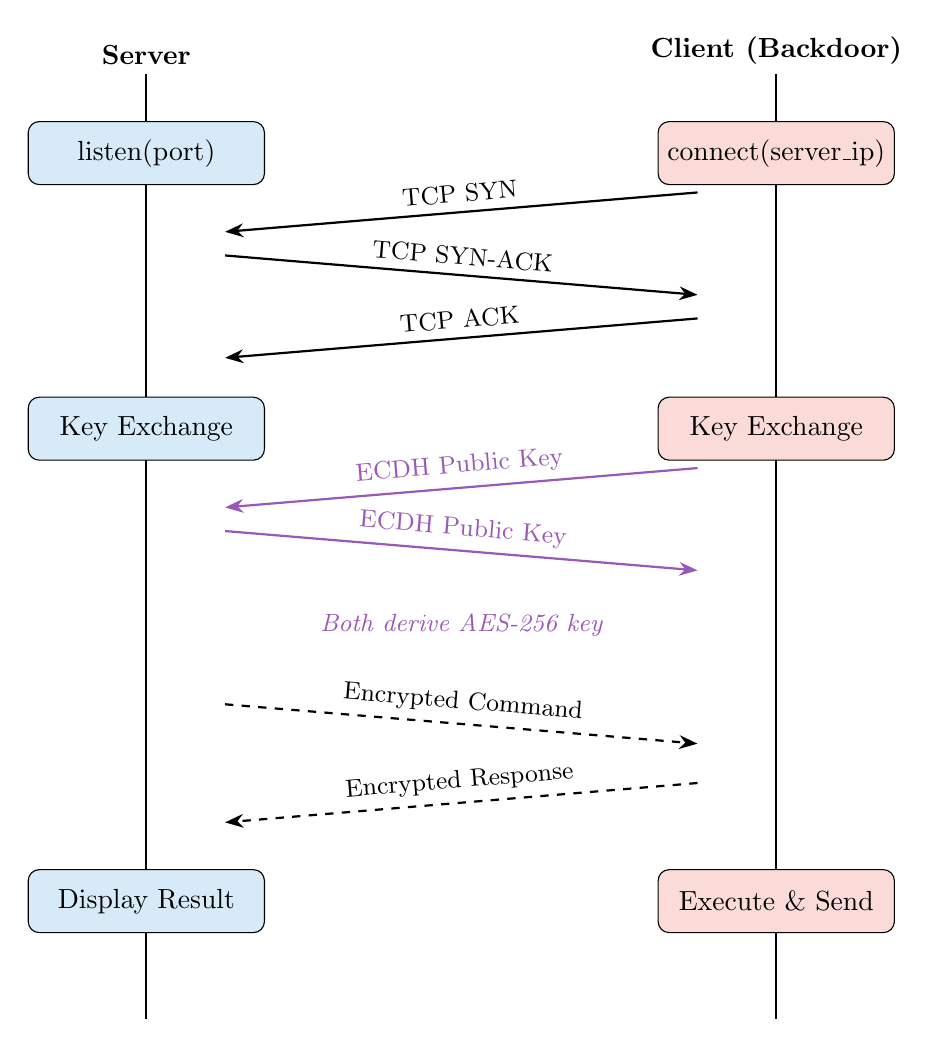
\begin{tikzpicture}[
    node distance=0.5cm,
    block/.style={rectangle, draw, minimum width=3cm, minimum height=0.8cm, rounded corners},
    serverblock/.style={block, fill=servercolor!20},
    clientblock/.style={block, fill=clientcolor!20}
]

% Timeline
\draw[thick] (0,0) -- (0,-12);
\draw[thick] (8,0) -- (8,-12);

\node[above] at (0,0) {\textbf{Server}};
\node[above] at (8,0) {\textbf{Client (Backdoor)}};

% Steps
\node[serverblock] at (0,-1) {listen(port)};
\node[clientblock] at (8,-1) {connect(server\_ip)};

\draw[-Stealth, thick] (7,-1.5) -- (1,-2) node[midway, above, sloped, font=\small] {TCP SYN};
\draw[-Stealth, thick] (1,-2.3) -- (7,-2.8) node[midway, above, sloped, font=\small] {TCP SYN-ACK};
\draw[-Stealth, thick] (7,-3.1) -- (1,-3.6) node[midway, above, sloped, font=\small] {TCP ACK};

\node[serverblock] at (0,-4.5) {Key Exchange};
\node[clientblock] at (8,-4.5) {Key Exchange};

\draw[-Stealth, thick, color=cryptocolor] (7,-5) -- (1,-5.5) node[midway, above, sloped, font=\small] {ECDH Public Key};
\draw[-Stealth, thick, color=cryptocolor] (1,-5.8) -- (7,-6.3) node[midway, above, sloped, font=\small] {ECDH Public Key};

\node[font=\small\itshape, color=cryptocolor] at (4,-7) {Both derive AES-256 key};

\draw[-Stealth, thick, dashed] (1,-8) -- (7,-8.5) node[midway, above, sloped, font=\small] {Encrypted Command};
\draw[-Stealth, thick, dashed] (7,-9) -- (1,-9.5) node[midway, above, sloped, font=\small] {Encrypted Response};

\node[serverblock] at (0,-10.5) {Display Result};
\node[clientblock] at (8,-10.5) {Execute \& Send};

\end{tikzpicture}
\caption{Connection and Communication Sequence}
\end{figure}

\subsection{Message Format}

Commands and responses are transmitted using a simple text-based protocol:

\begin{table}[H]
\centering
\begin{tabular}{lll}
\toprule
\textbf{Type} & \textbf{Format} & \textbf{Example} \\
\midrule
Simple Command & \texttt{command} & \texttt{ps}, \texttt{info}, \texttt{persist} \\
Parameterized & \texttt{command:param} & \texttt{kill:1234}, \texttt{wol:AA:BB:CC:DD:EE:FF} \\
File Transfer & \texttt{file:size:name:contents} & \texttt{file:1024:test.txt:data...} \\
Directory & \texttt{cd path} & \texttt{cd C:\textbackslash Users} \\
\bottomrule
\end{tabular}
\caption{Command Protocol Format}
\end{table}

\newpage
\section{Encryption System}

\subsection{Key Exchange (ECDH-P256)}

BlxdMoon uses Elliptic Curve Diffie-Hellman for secure key exchange:

\begin{figure}[H]
\centering
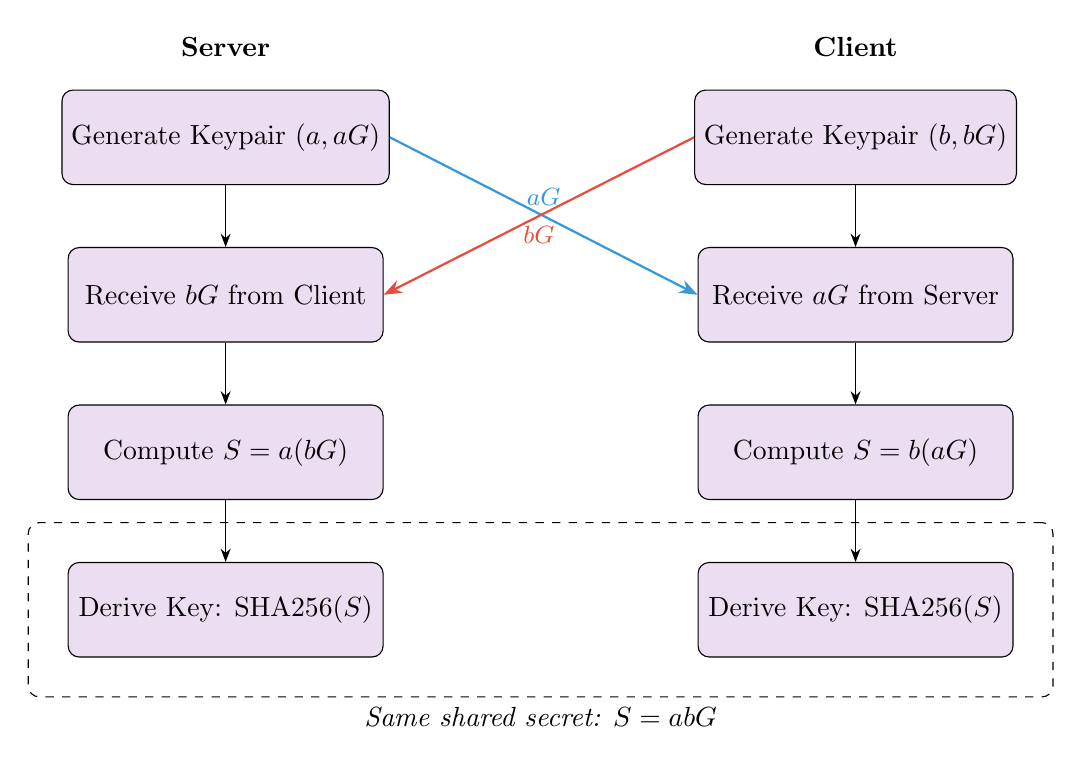
\begin{tikzpicture}[
    node distance=1cm,
    box/.style={rectangle, draw, minimum width=4cm, minimum height=1.2cm, rounded corners, fill=cryptocolor!20}
]

% Server side
\node[box] (s1) at (0,0) {Generate Keypair $(a, aG)$};
\node[box] (s2) at (0,-2) {Receive $bG$ from Client};
\node[box] (s3) at (0,-4) {Compute $S = a(bG)$};
\node[box] (s4) at (0,-6) {Derive Key: SHA256($S$)};

% Client side
\node[box] (c1) at (8,0) {Generate Keypair $(b, bG)$};
\node[box] (c2) at (8,-2) {Receive $aG$ from Server};
\node[box] (c3) at (8,-4) {Compute $S = b(aG)$};
\node[box] (c4) at (8,-6) {Derive Key: SHA256($S$)};

% Arrows
\draw[-Stealth] (s1) -- (s2);
\draw[-Stealth] (s2) -- (s3);
\draw[-Stealth] (s3) -- (s4);
\draw[-Stealth] (c1) -- (c2);
\draw[-Stealth] (c2) -- (c3);
\draw[-Stealth] (c3) -- (c4);

% Exchange arrows
\draw[-Stealth, thick, color=servercolor] (s1.east) -- node[above, font=\small] {$aG$} (c2.west);
\draw[-Stealth, thick, color=clientcolor] (c1.west) -- node[below, font=\small] {$bG$} (s2.east);

% Labels
\node[above=0.3cm of s1, font=\bfseries] {Server};
\node[above=0.3cm of c1, font=\bfseries] {Client};

% Shared secret indicator
\node[draw, dashed, rounded corners, inner sep=0.5cm, fit=(s4)(c4), label={below:\textit{Same shared secret: $S = abG$}}] {};

\end{tikzpicture}
\caption{ECDH Key Exchange Process}
\end{figure}

\subsection{Data Encryption (AES-256-CBC)}

After key exchange, all communication is encrypted:

\begin{lstlisting}[style=cstyle, caption={Encryption Process}]
// Message format: [IV (16 bytes)][Ciphertext][PKCS7 Padding]
int crypto_encrypt(const unsigned char *plaintext, int len,
                   unsigned char *ciphertext) {
    // 1. Generate random IV
    generate_random(session_iv, 16);

    // 2. Copy IV to output (first 16 bytes)
    memcpy(ciphertext, session_iv, 16);

    // 3. Apply PKCS7 padding
    int padded_len = ((len / 16) + 1) * 16;

    // 4. Encrypt with AES-256-CBC
    BCryptEncrypt(hKey, padded, padded_len, NULL,
                  iv_copy, 16, ciphertext + 16, ...);
}
\end{lstlisting}

\newpage
\section{Feature Modules}

\subsection{Process Management}

The process management module provides system reconnaissance capabilities:

\begin{figure}[H]
\centering
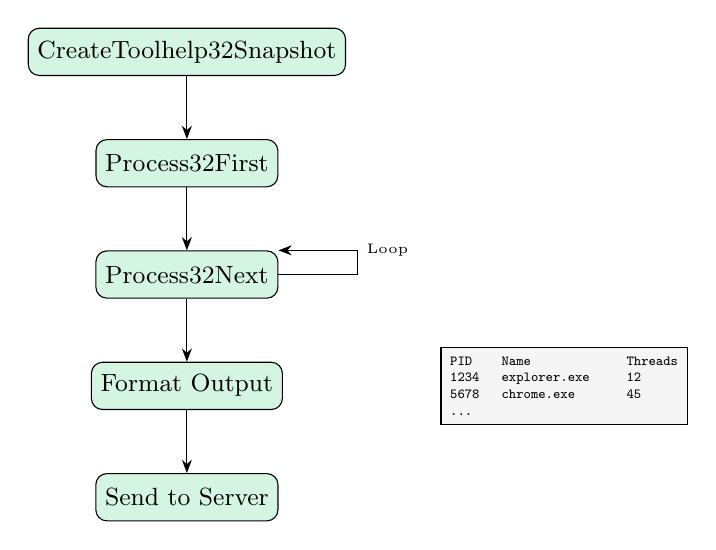
\begin{tikzpicture}[
    node distance=0.8cm,
    process/.style={rectangle, draw, minimum width=2cm, minimum height=0.6cm, rounded corners, fill=datacolor!20, font=\small}
]

\node[process] (snap) {CreateToolhelp32Snapshot};
\node[process, below=of snap] (first) {Process32First};
\node[process, below=of first] (next) {Process32Next};
\node[process, below=of next] (format) {Format Output};
\node[process, below=of format] (send) {Send to Server};

\draw[-Stealth] (snap) -- (first);
\draw[-Stealth] (first) -- (next);
\draw[-Stealth] (next) -- (format);
\draw[-Stealth] (format) -- (send);
\draw[-Stealth] (next.east) -- ++(1,0) |- (next.north east) node[midway, right, font=\tiny] {Loop};

% Output example
\node[right=2cm of format, draw, fill=codebg, font=\ttfamily\tiny, align=left] {
PID~~~~Name~~~~~~~~~~~~~Threads\\
1234~~~explorer.exe~~~~~12\\
5678~~~chrome.exe~~~~~~~45\\
...
};

\end{tikzpicture}
\caption{Process Enumeration Flow}
\end{figure}

\subsection{Keylogger Architecture}

\begin{figure}[H]
\centering
\begin{tikzpicture}[
    node distance=1cm,
    block/.style={rectangle, draw, minimum width=3cm, minimum height=1cm, rounded corners}
]

\node[block, fill=clientcolor!20] (main) {Main Thread (Shell)};
\node[block, fill=datacolor!20, right=3cm of main] (logger) {Logger Thread};
\node[block, fill=yellow!20, below=of logger] (file) {Temp File};

\draw[-Stealth] (main) -- node[above, font=\small] {CreateThread} (logger);
\draw[-Stealth] (logger) -- node[right, font=\small] {fputc(key)} (file);

% Keyboard
\node[left=1.5cm of logger] (kb) {\faKeyboard};
\draw[-Stealth] (kb) -- node[above, font=\tiny] {GetKeyState} (logger);

% Loop indicator
\draw[-Stealth] (logger.north) -- ++(0,0.5) -| ++(-0.5,0) |- (logger.west) node[midway, above, font=\tiny] {Sleep(10ms)};

\end{tikzpicture}
\caption{Keylogger Thread Architecture}
\end{figure}

\subsection{Browser Credential Extraction}

\begin{figure}[H]
\centering
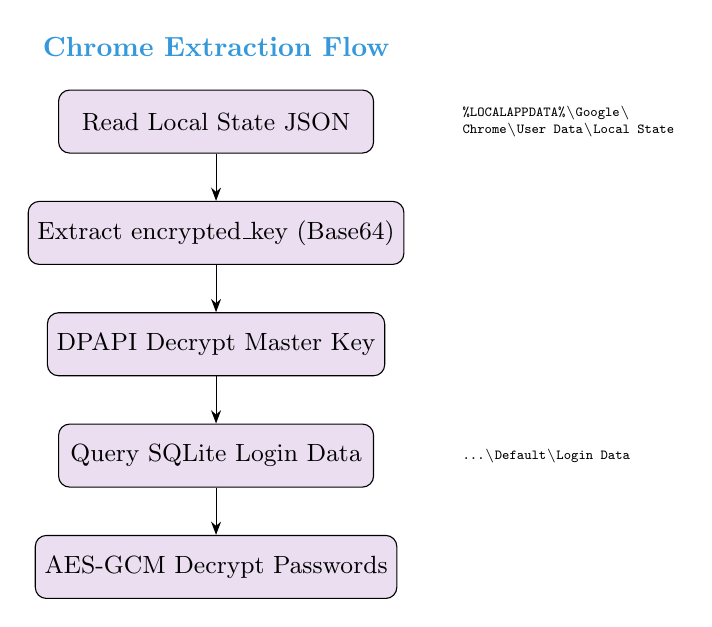
\begin{tikzpicture}[
    node distance=0.6cm,
    stepbox/.style={rectangle, draw, minimum width=4cm, minimum height=0.8cm, rounded corners, fill=cryptocolor!20, font=\small}
]

% Chrome flow
\node[stepbox] (c1) {Read Local State JSON};
\node[stepbox, below=of c1] (c2) {Extract encrypted\_key (Base64)};
\node[stepbox, below=of c2] (c3) {DPAPI Decrypt Master Key};
\node[stepbox, below=of c3] (c4) {Query SQLite Login Data};
\node[stepbox, below=of c4] (c5) {AES-GCM Decrypt Passwords};

\draw[-Stealth] (c1) -- (c2);
\draw[-Stealth] (c2) -- (c3);
\draw[-Stealth] (c3) -- (c4);
\draw[-Stealth] (c4) -- (c5);

\node[above=0.3cm of c1, font=\bfseries\color{servercolor}] {Chrome Extraction Flow};

% File paths
\node[right=1cm of c1, font=\ttfamily\tiny, align=left] {\%LOCALAPPDATA\%\textbackslash Google\textbackslash\\Chrome\textbackslash User Data\textbackslash Local State};
\node[right=1cm of c4, font=\ttfamily\tiny, align=left] {...\textbackslash Default\textbackslash Login Data};

\end{tikzpicture}
\caption{Chrome Credential Extraction Process}
\end{figure}

\newpage
\section{Multi-Client Server}

\subsection{Server Architecture}

The v2.0 server supports multiple simultaneous client connections:

\begin{figure}[H]
\centering
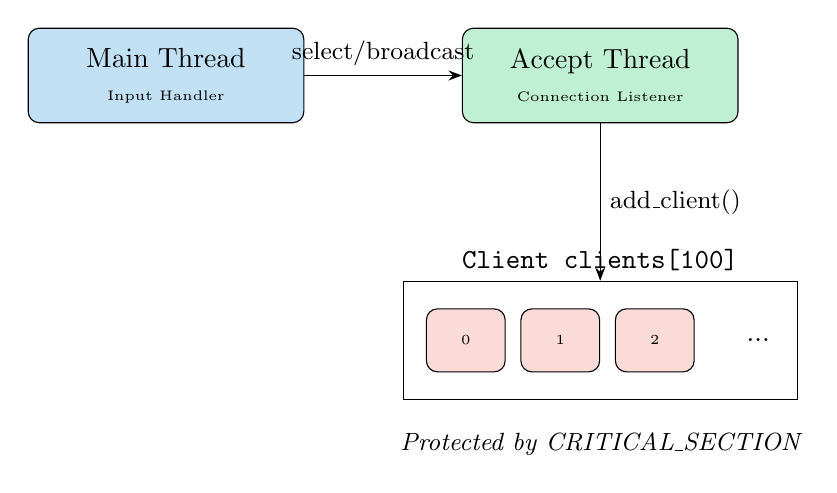
\begin{tikzpicture}[
    node distance=1cm,
    thread/.style={rectangle, draw, minimum width=3.5cm, minimum height=1.2cm, rounded corners, align=center},
    mainthread/.style={thread, fill=servercolor!30},
    acceptthread/.style={thread, fill=datacolor!30},
    clientthread/.style={thread, fill=clientcolor!20}
]

% Main thread
\node[mainthread] (main) {Main Thread\\\tiny Input Handler};

% Accept thread
\node[acceptthread, right=2cm of main] (accept) {Accept Thread\\\tiny Connection Listener};

% Client array
\node[draw, minimum width=5cm, minimum height=1.5cm, below=2cm of accept] (clients) {};
\node[above] at (clients.north) {\texttt{Client clients[100]}};

% Client boxes
\node[clientthread, minimum width=1cm, minimum height=0.8cm] at ($(clients.west)+(0.8,0)$) (c0) {\tiny 0};
\node[clientthread, minimum width=1cm, minimum height=0.8cm] at ($(clients.west)+(2,0)$) (c1) {\tiny 1};
\node[clientthread, minimum width=1cm, minimum height=0.8cm] at ($(clients.west)+(3.2,0)$) (c2) {\tiny 2};
\node at ($(clients.east)+(-0.5,0)$) {...};

% Arrows
\draw[-Stealth] (accept) -- node[right, font=\small] {add\_client()} (clients);
\draw[-Stealth] (main) -- node[above, font=\small] {select/broadcast} (accept);

% Critical section
\node[below=0.3cm of clients, font=\small\itshape] {Protected by CRITICAL\_SECTION};

\end{tikzpicture}
\caption{Multi-Client Server Threading Model}
\end{figure}

\subsection{Server Commands}

\begin{table}[H]
\centering
\begin{tabular}{llp{6cm}}
\toprule
\textbf{Command} & \textbf{Syntax} & \textbf{Description} \\
\midrule
\texttt{list} & \texttt{list} & Display all connected clients \\
\texttt{select} & \texttt{select <id>} & Enter interaction mode with client \\
\texttt{broadcast} & \texttt{broadcast <cmd>} & Send command to all clients \\
\texttt{kick} & \texttt{kick <id>} & Disconnect a specific client \\
\texttt{back} & \texttt{back} & Return to main menu (in client mode) \\
\texttt{exit} & \texttt{exit} & Shutdown server \\
\bottomrule
\end{tabular}
\caption{Server Management Commands}
\end{table}

\subsection{Interactive Menu}

\begin{tcolorbox}[title=Server Interface Example, colback=black!90, coltext=green!70!white, coltitle=white, fontupper=\ttfamily\small]
\textcolor{red}{=== BlxdMoon C2 Server ===}\\
Connected clients: 3\\
\\
~~[\textcolor{green}{0}] 192.168.1.100 - DESKTOP-ABC (admin) - 5m ago\\
~~[\textcolor{green}{1}] 192.168.1.105 - LAPTOP-XYZ (john) - 2m ago\\
~~[\textcolor{green}{2}] 192.168.1.110 - PC-HOME (user) - 30s ago\\
\\
\textcolor{yellow}{Commands:}\\
~~select <id>~~~~- Interact with a client\\
~~broadcast <cmd> - Send command to all\\
~~kick <id>~~~~~~- Disconnect a client\\
\\
\textcolor{red}{Blxd}\textcolor{green}{Moon}> select 0\\
\\
{[}*{]} Now interacting with client 0 (192.168.1.100)\\
\\
\textcolor{cyan}{client[0]}> ps
\end{tcolorbox}

\newpage
\section{Command Reference}

\subsection{All Available Commands}

\begin{longtable}{llp{5cm}}
\toprule
\textbf{Command} & \textbf{Category} & \textbf{Description} \\
\midrule
\endhead
\texttt{info} & Recon & System information (hostname, user, IP, CPU) \\
\texttt{ps} & Recon & List all running processes \\
\texttt{kill:<pid>} & Recon & Terminate process by PID \\
\midrule
\texttt{screen} & Surveillance & Capture screenshot (BMP) \\
\texttt{keylogger:start} & Surveillance & Start background keylogger \\
\texttt{clipboard:start} & Surveillance & Start clipboard monitor \\
\texttt{clipboard:dump} & Surveillance & Get current clipboard contents \\
\texttt{webcam} & Surveillance & Capture webcam frame \\
\texttt{webcam:list} & Surveillance & List available webcams \\
\midrule
\texttt{browser:creds} & Credentials & Extract all browser passwords \\
\texttt{browser:chrome} & Credentials & Extract Chrome passwords \\
\texttt{browser:firefox} & Credentials & Extract Firefox passwords \\
\midrule
\texttt{upload <file>} & File Transfer & Upload file to client \\
\texttt{download <file>} & File Transfer & Download file from client \\
\texttt{cd <dir>} & File Transfer & Change working directory \\
\midrule
\texttt{persist} & Persistence & Add registry autorun entry \\
\texttt{wol:<mac>} & Network & Send Wake-on-LAN packet \\
\texttt{q} & Control & Disconnect client \\
\texttt{<any>} & Shell & Execute shell command \\
\bottomrule
\caption{Complete Command Reference}
\end{longtable}

\newpage
\section{Persistence Mechanism}

BlxdMoon achieves persistence through Windows Registry modification:

\begin{figure}[H]
\centering
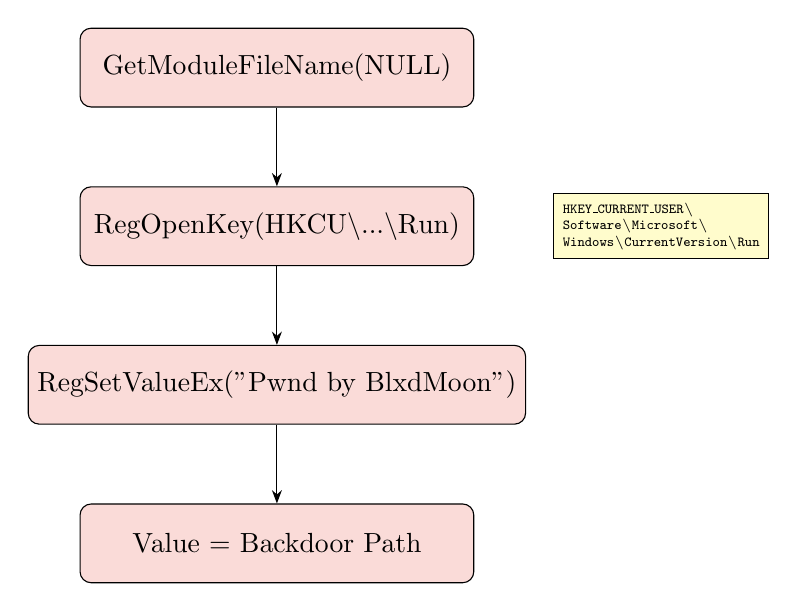
\begin{tikzpicture}[
    node distance=1cm,
    stepbox/.style={rectangle, draw, minimum width=5cm, minimum height=1cm, rounded corners, fill=clientcolor!20}
]

\node[stepbox] (s1) {GetModuleFileName(NULL)};
\node[stepbox, below=of s1] (s2) {RegOpenKey(HKCU\textbackslash...\textbackslash Run)};
\node[stepbox, below=of s2] (s3) {RegSetValueEx("Pwnd by BlxdMoon")};
\node[stepbox, below=of s3] (s4) {Value = Backdoor Path};

\draw[-Stealth] (s1) -- (s2);
\draw[-Stealth] (s2) -- (s3);
\draw[-Stealth] (s3) -- (s4);

\node[right=1cm of s2, draw, fill=yellow!20, font=\ttfamily\tiny, align=left] {
HKEY\_CURRENT\_USER\textbackslash\\
Software\textbackslash Microsoft\textbackslash\\
Windows\textbackslash CurrentVersion\textbackslash Run
};

\end{tikzpicture}
\caption{Registry Persistence Mechanism}
\end{figure}

\section{Data Flow Visualization}

\begin{figure}[H]
\centering
\begin{tikzpicture}[
    scale=0.85,
    transform shape,
    node distance=1cm,
    dataflow/.style={-Stealth, thick},
    encrypt/.style={-Stealth, thick, color=cryptocolor, dashed}
]

% Server
\node[draw, minimum width=3cm, minimum height=4cm, fill=servercolor!10] (server) {};
\node[above] at (server.north) {\textbf{C2 Server}};

% Server internal
\node[draw, fill=white, minimum width=2.5cm] at ($(server.north)+(0,-1)$) (input) {User Input};
\node[draw, fill=white, minimum width=2.5cm] at ($(server.center)$) (crypto1) {Encrypt};
\node[draw, fill=white, minimum width=2.5cm] at ($(server.south)+(0,1)$) (send1) {TCP Send};

% Network
\node[draw, ellipse, minimum width=2cm, fill=gray!20] at ($(server.east)+(2,0)$) (net) {\faCloud};

% Client
\node[draw, minimum width=3cm, minimum height=4cm, fill=clientcolor!10] at ($(net.east)+(2,0)$) (client) {};
\node[above] at (client.north) {\textbf{Backdoor}};

% Client internal
\node[draw, fill=white, minimum width=2.5cm] at ($(client.north)+(0,-1)$) (recv) {TCP Recv};
\node[draw, fill=white, minimum width=2.5cm] at ($(client.center)$) (crypto2) {Decrypt};
\node[draw, fill=white, minimum width=2.5cm] at ($(client.south)+(0,1)$) (exec) {Execute};

% Flows
\draw[dataflow] (input) -- (crypto1);
\draw[encrypt] (crypto1) -- (send1);
\draw[dataflow] (send1.east) -- (net);
\draw[dataflow] (net) -- (recv.west);
\draw[encrypt] (recv) -- (crypto2);
\draw[dataflow] (crypto2) -- (exec);

% Legend
\node[below=0.5cm of client.south, font=\small] {
    \tikz{\draw[-Stealth, thick] (0,0) -- (0.5,0);} Plaintext~~
    \tikz{\draw[-Stealth, thick, dashed, color=cryptocolor] (0,0) -- (0.5,0);} Encrypted
};

\end{tikzpicture}
\caption{Command Data Flow}
\end{figure}

\newpage
\section{Build System}

\subsection{CMake Configuration}

\begin{lstlisting}[style=bashstyle, caption={CMakeLists.txt (excerpt)}]
# Backdoor executable
add_executable(backdoor
    src/backdoor.c src/logger.c src/screen.c
    src/process.c src/clipboard.c src/browser.c
    src/webcam.c src/crypto.c ...
)

# Required Windows libraries
target_link_libraries(backdoor
    ws2_32      # WinSock2 networking
    gdi32       # Graphics (screenshots)
    bcrypt      # Cryptography (AES, ECDH)
    crypt32     # DPAPI (browser creds)
    strmiids    # DirectShow (webcam)
    ole32       # COM initialization
)
\end{lstlisting}

\subsection{Compilation Steps}

\begin{enumerate}
    \item \textbf{Configure IP/Port:}
    \begin{lstlisting}[style=bashstyle]
./configure.sh 192.168.1.100 4444
    \end{lstlisting}

    \item \textbf{Build with CMake:}
    \begin{lstlisting}[style=bashstyle]
mkdir build && cd build
cmake ..
make
    \end{lstlisting}

    \item \textbf{Output:}
    \begin{itemize}
        \item \texttt{build/server.exe} -- C2 Server
        \item \texttt{build/backdoor.exe} -- Client/Backdoor
    \end{itemize}
\end{enumerate}

\section{Conclusion}

BlxdMoon demonstrates fundamental RAT techniques including:

\begin{itemize}
    \item Client-server architecture with TCP sockets
    \item Windows API usage for system interaction
    \item Cryptographic protocols for secure communication
    \item Multi-threading for concurrent operations
    \item Persistence through registry modification
    \item Credential harvesting techniques
\end{itemize}

\begin{infobox}
This analysis is provided for educational purposes to understand malware techniques and improve defensive security measures. The knowledge gained should be applied to develop better detection and prevention mechanisms.
\end{infobox}

\newpage
\appendix
\section{File Structure}

\begin{verbatim}
BlxdMoon/
+-- CMakeLists.txt
+-- configure.sh
+-- include/
|   +-- browser.h
|   +-- clipboard.h
|   +-- crypto.h
|   +-- logger.h
|   +-- process.h
|   +-- screen.h
|   +-- status.h
|   +-- str_cut.h
|   +-- uuid.h
|   +-- webcam.h
|   +-- wol.h
+-- src/
|   +-- backdoor.c      (Main client)
|   +-- server.c        (C2 server)
|   +-- browser.c       (Credential extraction)
|   +-- clipboard.c     (Clipboard monitor)
|   +-- crypto.c        (ECDH + AES)
|   +-- logger.c        (Keylogger)
|   +-- process.c       (Process management)
|   +-- screen.c        (Screenshots)
|   +-- webcam.c        (Camera capture)
|   +-- ...
+-- repo/
    +-- banner.png
\end{verbatim}

\section{Dependencies}

\begin{table}[H]
\centering
\begin{tabular}{llp{5cm}}
\toprule
\textbf{Library} & \textbf{Header} & \textbf{Purpose} \\
\midrule
ws2\_32 & winsock2.h & TCP/IP networking \\
gdi32 & wingdi.h & Screen capture \\
bcrypt & bcrypt.h & ECDH, AES, SHA-256 \\
crypt32 & dpapi.h & DPAPI decryption \\
strmiids & dshow.h & DirectShow GUIDs \\
ole32 & objbase.h & COM initialization \\
\bottomrule
\end{tabular}
\caption{Windows Library Dependencies}
\end{table}

\end{document}
